\chapter{Obstacles Encountered}

\section{Description}
In this section, we discuss the obstacles associated with this project that led to delays in development and different solutions to be created from our original design.

\section{SensorTag}
The main obstacles we encountered within our design involved the SensorTag device from Texas Instruments. In trying to use the Zigbee firmware, we were unable to communicate between the SensorTag and XBee. Using SensorTag’s SmartRF Packet Sniffer 2 software, we were able to configure the SensorTag as a sniffer module. We found the packets to be very different from one another. In the SensorTag packet (Figure \ref{fig:sensortag}), it is very simple with a length value, sequence number, and data following the start frame delimiter. The XBee packet (Figure \ref{fig:xbee}) looks largely different. The packet is shown in hex as some values are not human-readable. It starts with a sequence number (0x1d), has various hex values, and then data (0x61 - 0x65). Even more peculiar, we find there to be a second sequence number (0x08). The data between the sequence numbers is unknown to us. With a few parameter changes to the XBee we are able to modify the packet a little bit but we were unable to have it coincide with the SensorTag’s packet which was not modifiable.

\begin{figure}[h]
  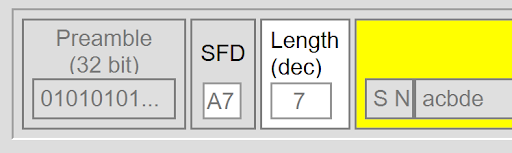
\includegraphics[width=0.8\textwidth]{SensorTag-packet.png}
  \centering
  \caption{SensorTag 802.15.4 Packet}
  \label{fig:sensortag}
\end{figure}

\begin{figure}[h]
  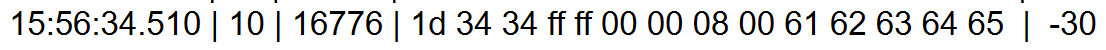
\includegraphics[width=0.9\textwidth]{XBee-packet.PNG}
  \centering
  \caption{XBee 802.15.4 Packet}
  \label{fig:xbee}
\end{figure}

We decided that it might be possible to use Bluetooth instead. The SensorTag could connect directly to the Raspberry Pi Zero W and reduce a cost of our system by not using the XBee. Unfortunately, we found SensorTag to be a difficult device to program. The IDE had a steep learning curve and documentation was difficult. Changes in documentation were not always reflected elsewhere causing confusion.

\section{XBee}
We encountered some confusion with XBee similarly to the SensorTag. There are two main variants to XBee that we were looking at: the S1 and S2C. It seemed like the S2C was an updated module but instead it was designed for mesh network implementations, which was unnecessary for our design. It was also thought that the XBee S1 could communicate with the S2C variant. That was not the case. The reasoning was unclear but it appears that some of the hardware configuration is different at the Mac layer; thus, the two could not interpret the data of the other. This cost us many delays as we had to wait for more modules to ship to us in these cases and when once module was defective. In buying 5 XBees, one was defective. Hopefully, this is not indicative of the reliability of these modules.